\section{Molecular Biology Background} \label{molecular-back-sect}
Epigenetics is a relatively new scientific field in Molecular Biology, and it describes the study of dynamic alterations in the transcriptional regulation of a cell. We can think of the epigenome as an external layer of information onto the genomic sequence, which can be used to understand major cellular processes, such as transcription, splicing and replication \citep{Furey2012}.

Regulation of gene expression in higher eukaryotic organisms depends on sequences within the DNA itself known as \emph{promoters}, and on a network of regulatory proteins, called \emph{transcription factors} (TFs) \citep{Jasny2001}. TFs are proteins that bind to specific DNA sequences, which are associated with specific genes, and facilitate of inhibit the recruitment of RNA polymerase in the promoter region of those genes \citep{Ptashne2002}. 

Recent advances in epigenetics have suggested some other mechanisms that regulate gene expression, such as the changes of the accessibility of the DNA, e.g. \emph{histone modifications} (HMs), and \emph{DNA methylation}. Histones are proteins that act as a spool where DNA can be wrapped around them to form \emph{nucleosomes}. The combination of DNA and nucleosomes within the nucleus of eukaryotic cells is called the \emph{chromatin}. 

DNA methylation is an epigenetic mark which occurs when a methyl group is attached to the \emph{cytosine} DNA nucleotides. In mammals, which we are mostly interested in this project, DNA methylation is observed almost exclusively on cytosines in the context of CpG dinucleotides (i.e. C followed by G, where p stands for the phosphate group between C and G). Genome wide CpGs are depleted, but mainly near promoter regions there are clusters of CpGs, which are called CpG islands (CGIs) \citep{Bird2002}. 

Owing to the rapid development of Next Generation Sequencing (NGS) technology, it is reasonable to expect genome sequences and other forms of high-throughput data to be measured extensively. For example, \emph{RNA-Seq} experiments \citep{Wang2009} are widely used for transcriptome profiling, i.e. measuring the set of all RNA molecules produced in a given cell or cell population (at a given time). \emph{Chip-Seq} experiments \citep{Park2009} are used to quantitatively measure and analyse protein interactions with DNA, i.e. HMs and binding of TFs. Whole-Genome Bisulphite Sequencing (WGBS) \citep{Frommer1992}, and Reduced Representation Bisulphite Sequencing (RRBS) \citep{Meissner2008}, are methods that use bisulphite treatment of DNA and allow estimation of methylation proportions at a single-nucleotide resolution. These are only some examples of the different platforms and techniques that are used to measure diverse biological components and are shown in \emph{Fig. \ref{seq-pic}}. 

\begin{figure}[h]
\begin{center}
 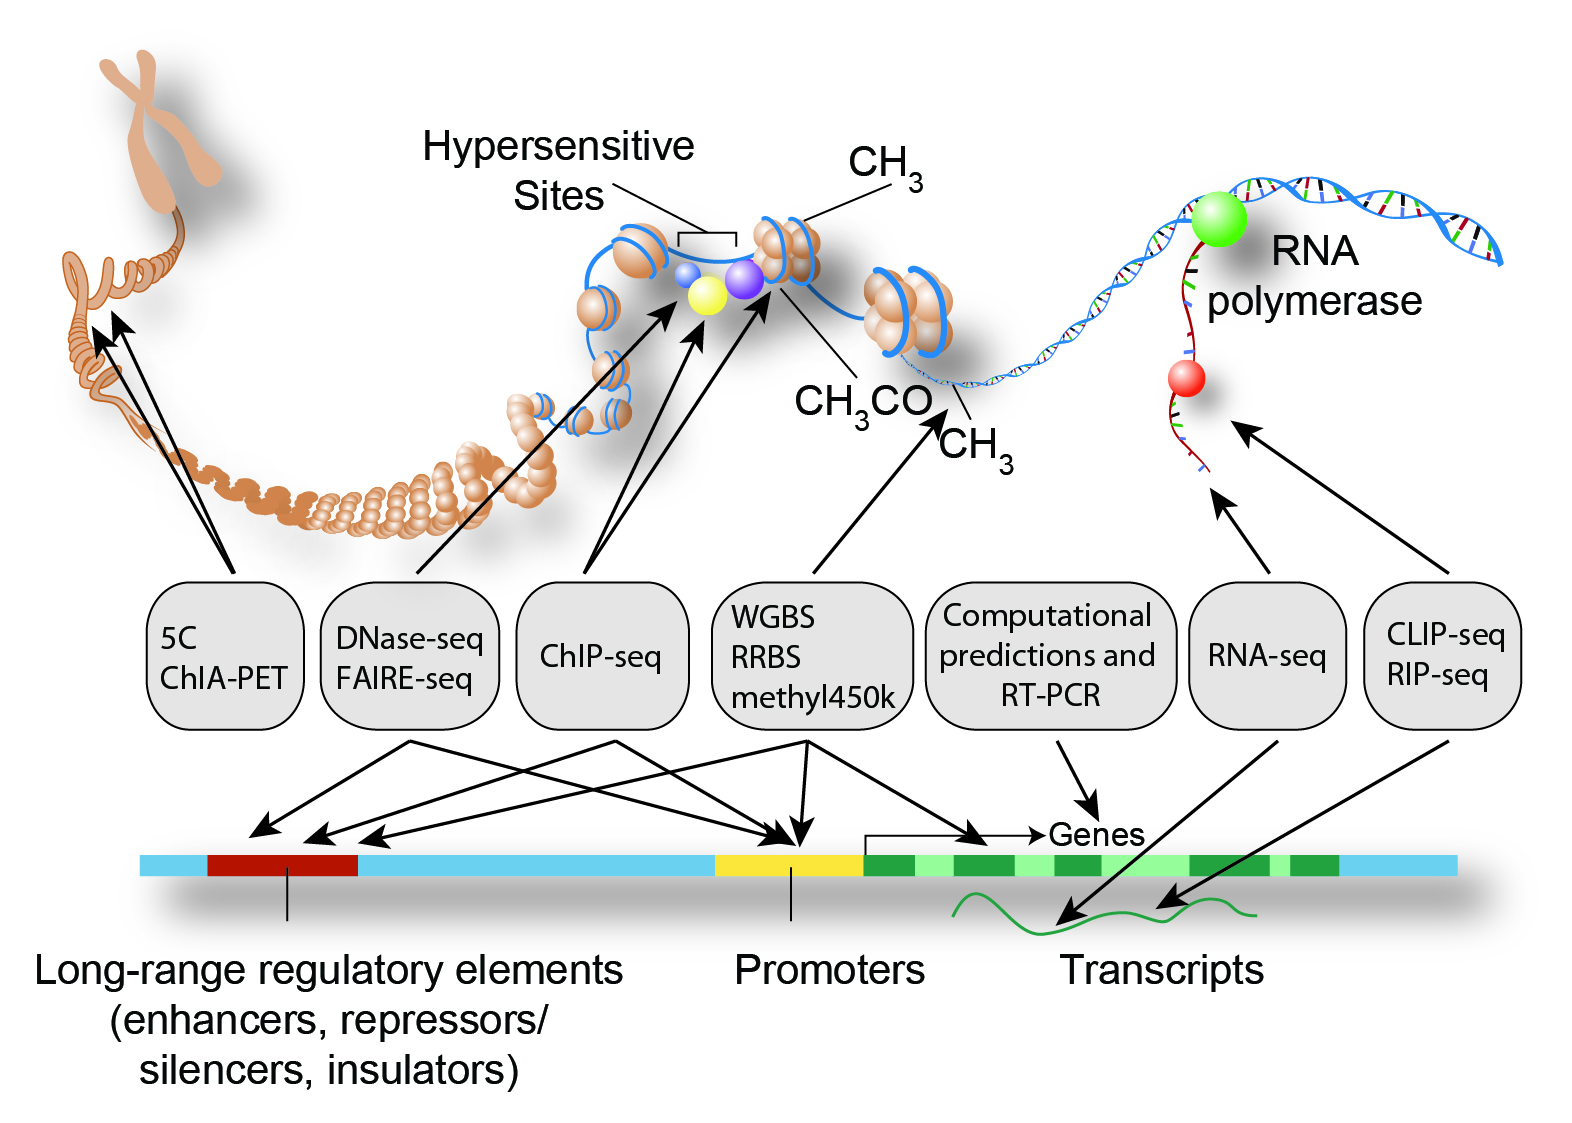
\includegraphics[scale = 0.15]{images/encode-seq.png}
\caption{\emph{Some of the XX-Seq techniques used from the ENCODE projet. Credits: Darryl Leja (NHGRI), Ian Dunham (EBI), Michael Pazin (NHGRI) \citep{Dunham2012}.}}
\label{seq-pic}
\end{center}
\end{figure} 

Recent research studies, assisted by whole-genome data analysis, demonstrated that gene expression and histone modifications (HMs) are well correlated, since a probabilistic model was created, which given a small number of HMs it could predict gene expression \citep{Karlic2010}. Also, \citep{Benveniste2014}, using the richness of the ENCODE datasets \citep{Dunham2012}, learned a logistic regression classifier with the TFs as input features and showed that only from knowledge of TF binding patterns at promoters they could accurately predict HMs. These are only some studies that show the correlation between genetic and epigenetic mechanisms. 

From the aforementioned, it is evident that in order to uncover and interpret the biological regulatory mechanisms an integrative analysis of these heterogeneous biomedical datasets should be performed, since by performing separate analyses of each data source we may not capture important associations between them.